
\chapter{An?lisis espacial. Fundamentos}



\pagestyle{fancy}

El an?lisis espacial es una de las tareas fundamentales sin las cuales el concepto de SIG no alcanza su verdadero significado. 

El an?lisis espacial es el \textbf{estudio cuantitativo de aquellos fen?menos que se manifiestan en el espacio}. Ello indica una importancia clave de la posici?n, la superficie, la distancia y la interacci?n a trav?s del propio espacio. 

Ejemplos de an?lisis que realizamos con cartograf?a fuera de un SIG son el buscar en un mapa d?nde se sit?a el pico m?s alto, ver la elevaci?n concreta a la que se encuentra un elemento dado tal como una poblaci?n, o planificar una jornada tur?stica viendo qu? lugares de inter?s podemos visitar o c?mo llegar desde uno a otro de estos lugares haci?ndolo por las mejores carreteras o de la forma m?s r?pida. Estas actividades habituales son ejemplos de an?lisis geogr?ficos que podemos igualmente realizar dentro de un SIG.

Mediante el an?lisis podemos generar nuevos datos que pueden ser \textbf{nuevas capas de datos geogr?ficos, tablas de datos, valores escalares} o \textbf{vectores}.

En ocasiones, los resultados expresan \textbf{la misma variable} que el dato de partida (por ejemplo, el c?lculo de una media), y en otros \textbf{las variables de entrada y salida son distintas} (por ejemplo, si a partir de una capa de elevaciones calculamos una de pendientes).

Asimismo, todo an?lisis espacial parte de un conjunto de datos espaciales, pudiendo estos ser \textbf{de un ?nico tipo, o de varios distintos} que se combinan en un procedimiento concreto. Por ejemplo, en el caso de calcular la localizaci?n del punto m?s alto, el resultado es una sencilla coordenada, y tan solo se utiliza la variable elevaci?n. En el caso de la altura media de una ciudad, se utilizan dos entradas: por un lado, la elevaci?n, y por otro, el emplazamiento de la ciudad. Aunque un mapa cl?sico contiene toda esa informaci?n en una ?nica hoja, en realidad son dos elementos distintos combinados a la hora de representarlos. En t?rminos m?s acordes con un SIG, podemos decir que tenemos dos capas distintas que utilizamos como entradas.

El an?lisis dentro un SIG nos permite tanto formular como responder a cuestiones. Estas cuestiones pueden ser:

\begin{itemize}
 \item Relativas a posici?n y extensi?n
\item Relativas a la forma y distribuci?n
\item Relativas a la asociaci?n espacial
\item Relativas a la interacci?n espacial
\item Relativas a la variaci?n espacial
\end{itemize}

\section{Algunos ejemplos de an?lisis espacial}

Algunos ejemplos de an?lisis espacial son los siguientes.

\subsection{Consulta espacial}

Vimos las consultas en detalle dentro del cap?tulo dedicado a las bases de datos.

Pueden combinarse con otros de los an?lisis disponibles, por ejemplo para la \textbf{selecci?n} de una serie de elementos sobre los que posteriormente se desarrollara el an?lisis en cuesti?n.

\subsection{An?lisis topol?gico}

Pueden plantearse consultas referidas no solo a la posici?n de los elementos geogr?ficos, sino a la \textbf{relaci?n con otros elementos}. La existencia de topolog?a puede emplearse para la realizaci?n de consultas que respondan a cuestiones como:

\begin{itemize}
\item ?C?mo llegar desde mi posici?n actual hasta una coordenada concreta por la red viaria existente?

\item ?Qu? comunidades aut?nomas comparten l?mite con Madrid?
\end{itemize}

\subsection{Medici?n} 

La existencia de una referencia espacial para cada uno de los elementos con los que trabajamos en el an?lisis dentro de un SIG hace que podamos \textbf{cuantificar} otra serie de par?metros tambi?n espaciales. Entre las mediciones m?s b?sicas, encontramos las distancias, ?reas, per?metros o factores de forma. Mas elaboradas, encontramos otras como pendientes o indices derivados de medidas simples.


\subsection{Combinaci?n}

Uno de los procedimientos m?s habituales y m?s caracter?sticos dentro del uso de un SIG es la \textbf{combinaci?n o superposici?n} de varias capas de informaci?n. La propia estructura de la informaci?n geogr?fica en capas facilita notablemente estos procedimientos y convierte a los SIG en plataformas ideales para llevar a cabo an?lisis donde se combina informaci?n sobre diversas variables.

En el caso de capas vectoriales, las \textbf{operaciones de solape} tales como \textbf{uni?n, intersecci?n, diferencia o recorte}, son habituales. La figura \ref{Fig:Interseccion} muestra un ejemplo de la operaci?n de intersecci?n con dos capas de pol?gonos.

\begin{figure}[!hbt]   
\centering
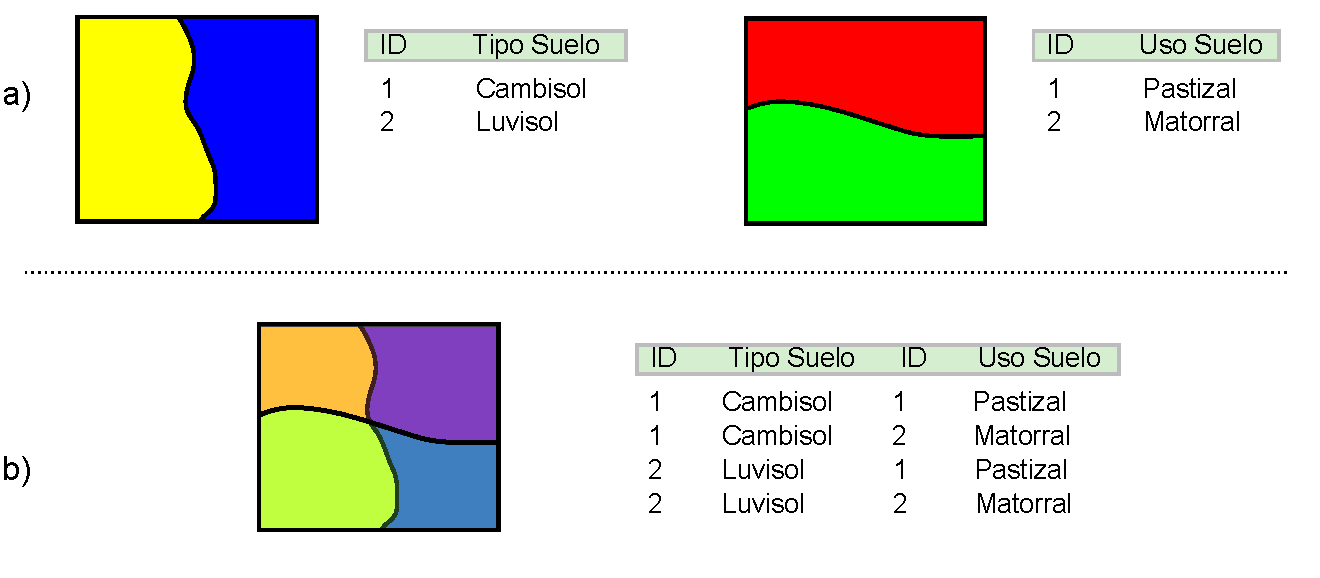
\includegraphics[width= \columnwidth]{../es/Analisis/Interseccion.pdf}
\caption{\small Operaci?n de intersecci?n de dos capas de pol?gonos.}
\label{Fig:Interseccion} 
\end{figure}

\subsection{Transformaciones}

Podemos englobar dentro de este grupo una amplia serie de procedimientos que modifican los elementos de entrada de diversas formas. Entre los m?s habituales, encontramos la \textbf{transformaci?n de coordenadas}, la \textbf{simplificaci?n de geometr?as}, o la \textbf{creaci?n de ?reas de influencia} o la \textbf{reclasificaci?n de valores}. Estas transformaci?n pueden afectar tanto a la componente espacial como a la componente tem?tica del dato. 

Un caso particular, ya mencionado en un cap?tulo anterior, es la \textbf{conversi?n entre modelos de datos}, esto es, entre el modelo r?ster y el vectorial. La figura \ref{Fig:Conversiones} muestra un ejemplo de esto. Partiendo de un mapa escaneado (una capa r?ster) con curvas de nivel, pueden detectarse estas y crearse una capa vectorial con dichas curvas de nivel. Estas pueden posteriormente convertirse en un Modelo Digital de Elevaciones (r?ster) mediante \textbf{interpolaci?n}, el cual es posible convertir de nuevo en una capa vectorial de l?neas.

\begin{figure}[!hbt]   
\centering
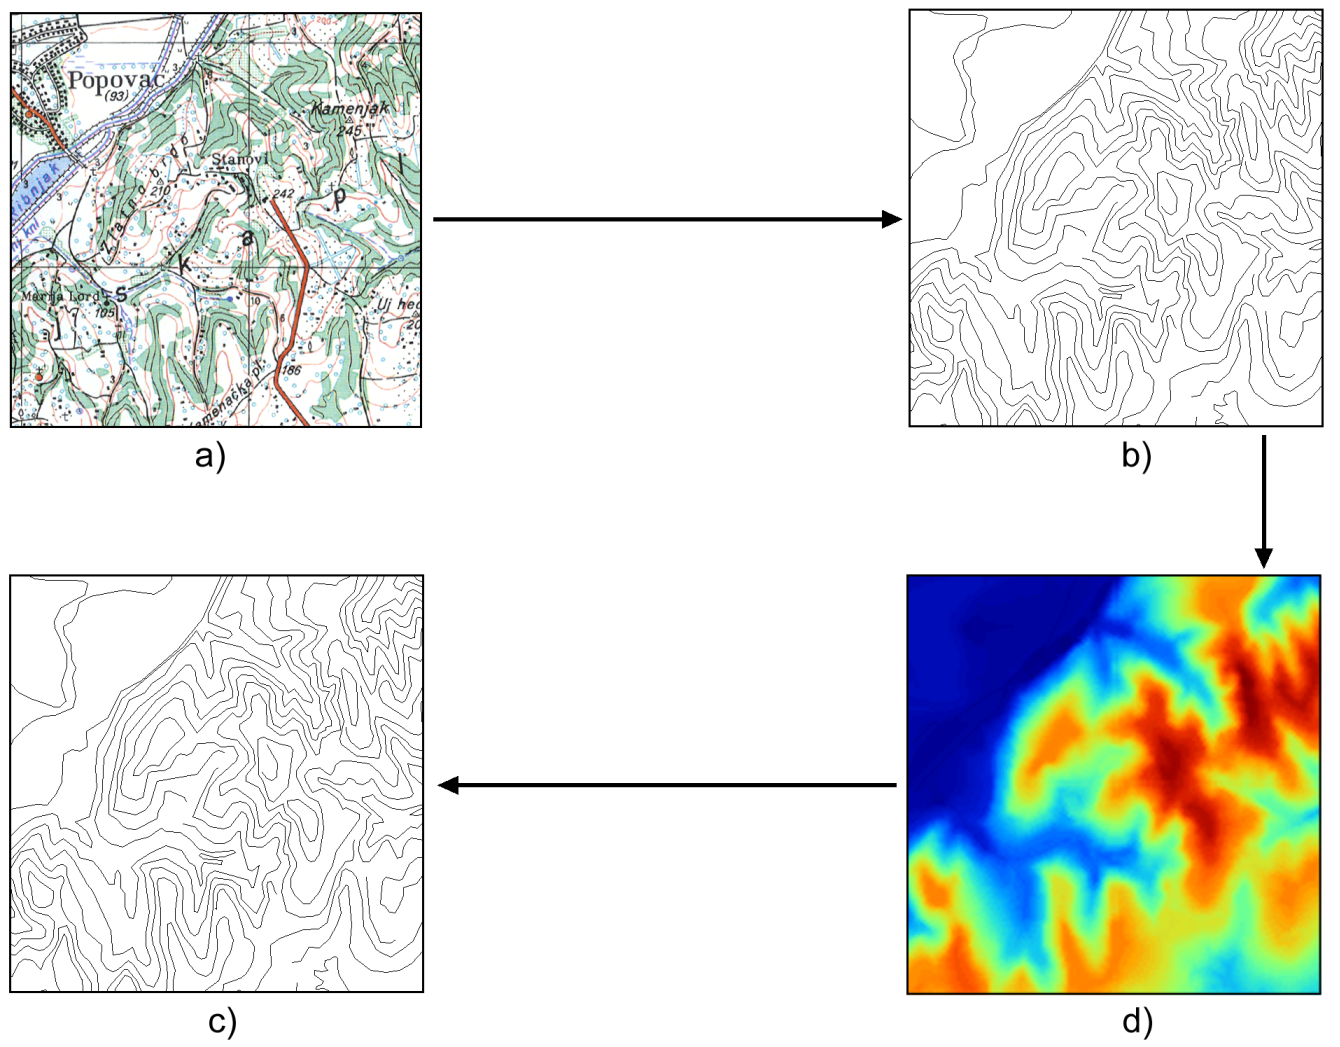
\includegraphics[width= \columnwidth]{../es/Analisis/Conversiones.png}
\caption{\small Conversi?n entre distintos modelos de datos para una capa de elevaciones.}
\label{Fig:Conversiones} 
\end{figure}

\subsection{An?lisis de superficies}

El an?lisis de superficies es uno de los m?s potentes de cuantos encontramos en un SIG. Desde par?metros b?sicos como la \textbf{pendiente} o la \textbf{orientaci?n} hasta par?metros morfom?tricos muy espec?ficos, pasando por todas las herramientas del \textbf{an?lisis hidrol?gico}, la bater?a de operaciones disponibles es muy amplia. 

\subsection{Estad?stica descriptiva}

Los elementos de la estad?stica cl?sica tienen sus equivalentes en los datos espaciales, y nos permiten \textbf{calificar cuantitativamente} los datos con los que trabajamos. Se incluyen aqu? descriptores de centralidad y dispersi?n, de dependencia espacial o el estudio de patrones espaciales, entre otros muchos. Estos pueden a su vez usarse para el contraste de hip?tesis que contengan una cierta componente espacial.

Por ejemplo, estos estad?sticos nos permiten dar respuesta a cuestiones del tipo:

\begin{itemize}
\item ?Es constante la media de altura a lo largo de toda la geograf?a de mi pa?s?

\item ?Existe alguna direcci?n predominante en los movimientos de individuos de una especie o se desplazan err?ticamente?
\end{itemize}

\subsection{Inferencia}

Otro an?lisis estad?stico de gran importancia en los SIG es el que permite inferir comportamientos de las distintas variables y estudiar, por ejemplo, la forma en que estas van a evolucionar a lo largo del tiempo.

El establecimiento de modelos de cambio y variaci?n representa una de las herramientas m?s actuales en el campo de los SIG, y un campo en abundante desarrollo.

\subsection{Toma de decisiones y optimizaci?n}

La estructura de la informaci?n geogr?fica en capas dentro de un SIG, favorable como ya vimos para la superposici?n de capas, lo es igualmente para estudiar de forma combinada los efectos de distintos factores. Este estudio nos permite luego responder a cuestiones como, por ejemplo:

\begin{itemize}
\item ?Cu?l es el mejor lugar para emplazar una nueva construcci?n en funci?n de su impacto sobre el medio?

\item ?D?nde situar un nuevo hospital para que el servicio en la comarca mejore lo m?ximo posible?
\end{itemize}

\subsection{Modelizaci?n}

La creaci?n de modelos espaciales dentro de un SIG es una tarea a?n pendiente de mucho desarrollo. No obstante, existe un gran n?mero de modelos en los m?s diversos campos, y la arquitectura de datos y procesos de los SIG es propicia para la implementaci?n de otros nuevos.


\section{Particularidades de los datos espaciales para su an?lisis}

Las caracter?sticas propias de los datos espaciales dotan a estos de una \textbf{gran potencialidad} de an?lisis, al tiempo que \textbf{condicionan o limitan} otras operaciones. Algunas de estas caracter?sticas representan problemas que han de tenerse presentes en el an?lisis; otros son simplemente conceptos b?sicos que deben conocerse pero no han de implicar necesariamente una dificultad asociada.

\subsection{Escala}


A la hora de estudiar la informaci?n geogr?fica, podemos hacerlo a \textbf{distintos niveles} y, dependiendo del nivel elegido, los resultados ser?n de una u otra naturaleza. Debido a esto, adem?s de considerar la escala cartogr?fica para la representaci?n y gesti?n de datos en un SIG, es necesario considerar la \textbf{escala de an?lisis}.

La escala de an?lisis depende \textbf{del dato en s?} (precisi?n, tipo, etc.), as? como del \textbf{an?lisis que se va a realizar} con ?l.

Como se muestra en la figura \ref{Fig:Escalas_formas_terreno}, si para definir las formas de relieve en un punto dado lo hacemos considerando dicho punto y los valores de elevaci?n a su alrededor, la caracterizaci?n que hagamos var?a en funci?n de la dimensi?n de esa zona alrededor (que es la que define la escala de an?lisis). Para valores peque?os de dicha zona de an?lisis, el punto analizado puede definirse como una cima, mientras que aumentando la escala de an?lisis se advierte que el punto se sit?a en el fondo de un valle.

\begin{figure}[h]   
\centering
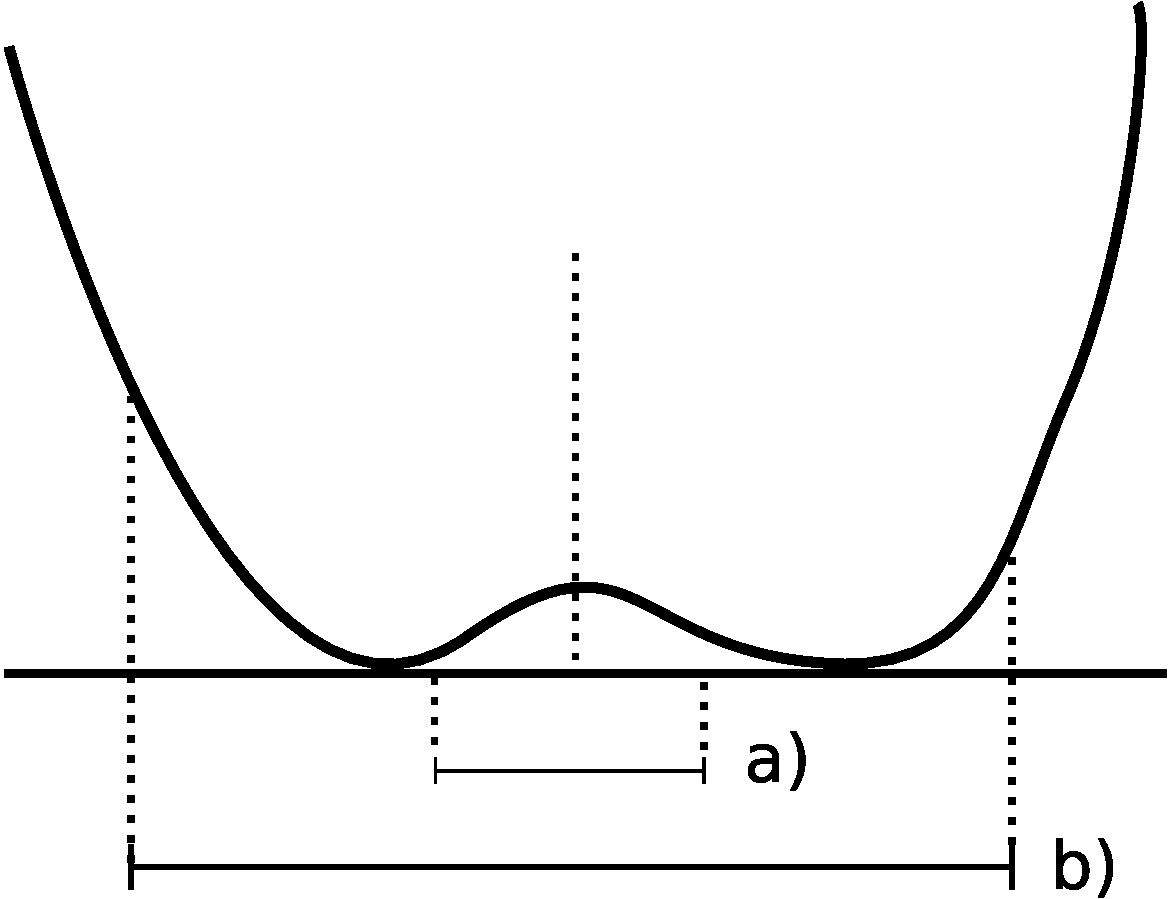
\includegraphics[width= .45\columnwidth]{../es/Analisis/Escalas_formas_terreno.pdf}
\caption{\small Dependiendo de la escala de an?lisis, un mismo relieve puede ser caracterizado como cima (a) o fondo de valle (b)}
\label{Fig:Escalas_formas_terreno} 
\end{figure}

Por tanto, debemos observar el relieve desde la distancia correcta a la cual la informaci?n que nos proporciona es la m?s adecuada para un an?lisis dado. Adem?s de existir una escala de mayor relevancia para un an?lisis concreto,  es de inter?s el trabajar a \textbf{m?ltiples escalas} y combinar los resultados.

Otro ejemplo de c?mo la escala de an?lisis condiciona los resultados obtenidos lo encontramos en el caso de efectuar \textbf{mediciones}. Como puede verse en la figura \ref{Fig:Medida_linea_fractal}, la unidad de medida empleada provoca que se obtengan resultados distintos. 

\begin{figure}[h]   
\centering
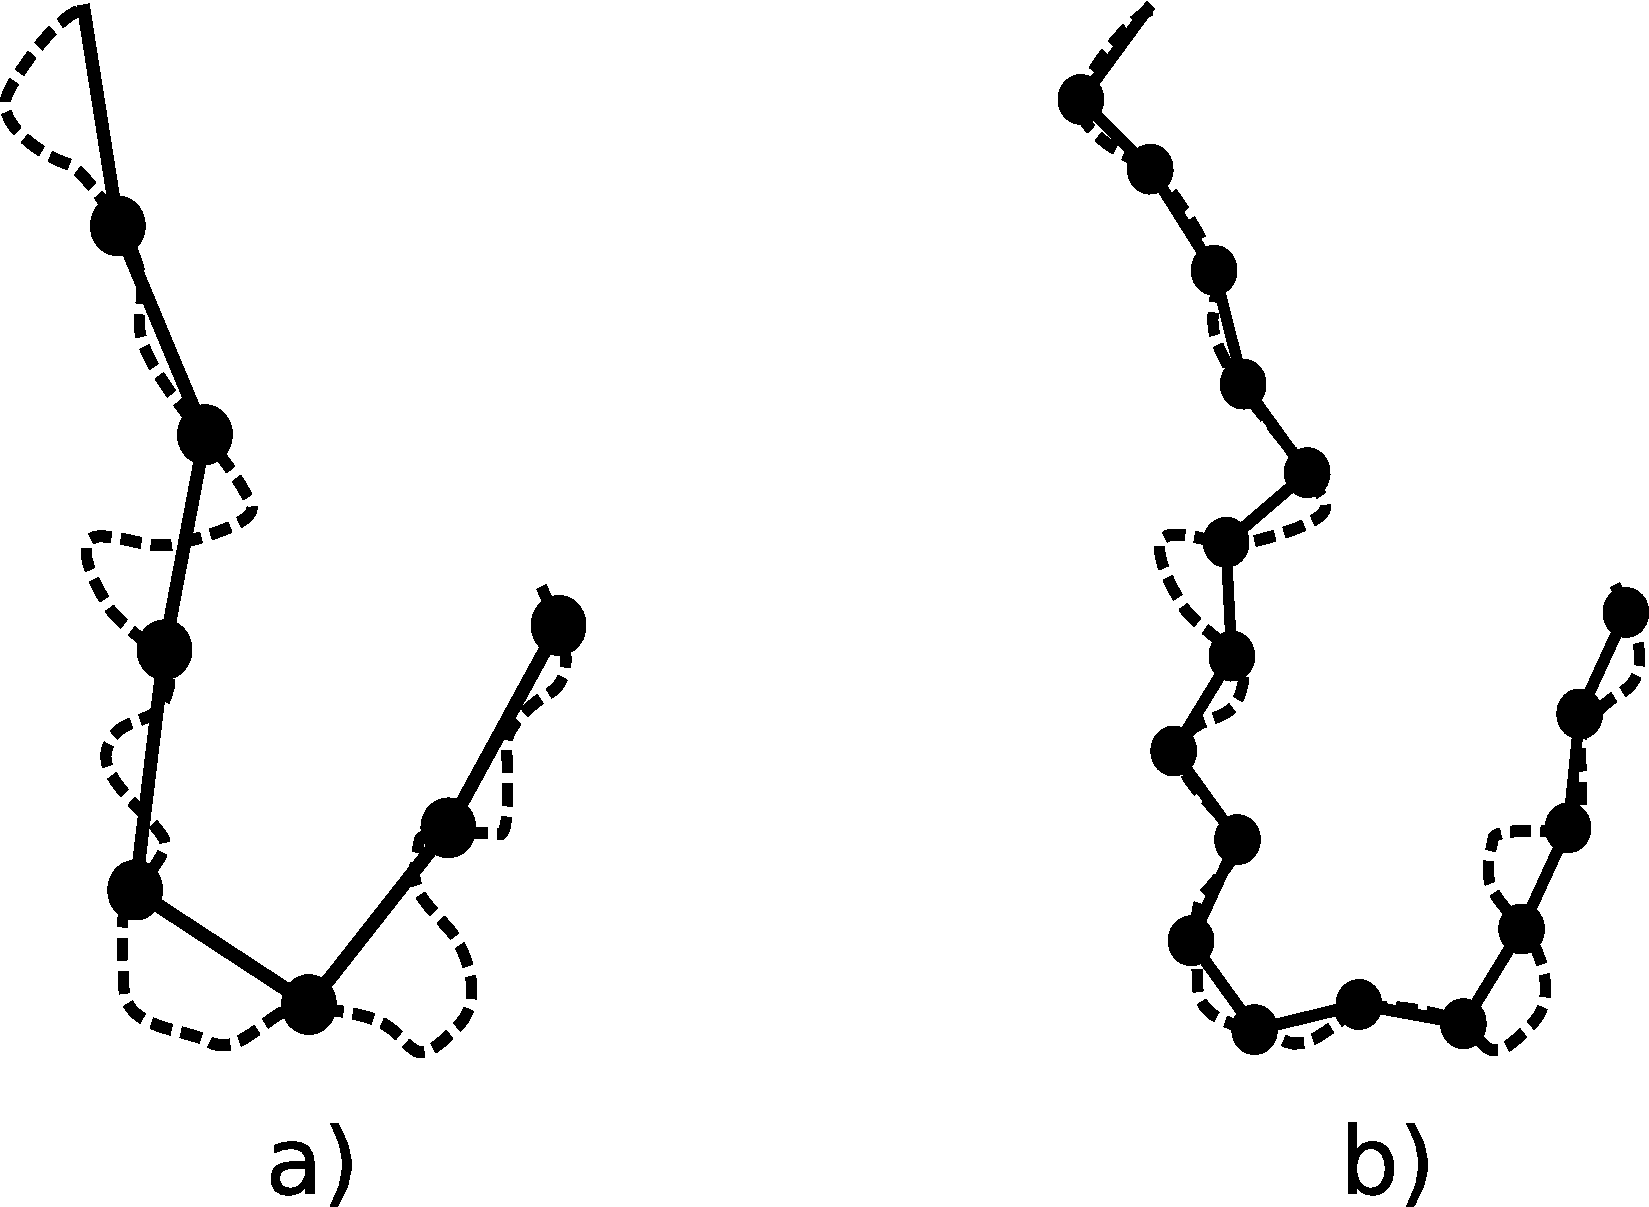
\includegraphics[width= .45\columnwidth]{../es/Analisis/Medida_linea_fractal.pdf}
\caption{\small La unidad de medida empleada modifica el resultado obtenido.}
\label{Fig:Medida_linea_fractal} 
\end{figure}

La uni?n del valor resultante con la escala a la que se ha obtenido tiene en conjunto pleno significado, pero ese valor por s? mismo carece de dicho significado. 

El concepto de \textbf{fractal} tiene una implicaci?n directa en este hecho.

El propio \textbf{formato de almacenamiento} condiciona el efecto de la escala, ya que puede imponer l?mites. Tal es el caso cuando se trabaja con capas raster, en las que el \textbf{tama?o de celda} delimita la precisi?n que puede obtenerse en el an?lisis.

\subsection{El Problema de la Unidad de ?rea Modificable}

Muchas de las variables con las que trabajamos dentro de un SIG \textbf{no pueden medirse de forma puntual}, y por ello han de \textbf{estudiarse para un ?rea dada}. Ejemplos de este tipo de variables son el porcentaje de poblaci?n en un rango de edad determinado o la densidad media de poblaci?n.

Las ?reas que se definen para poder trabajar con las variables de esta ?ndole son \textbf{esencialmente arbitrarias}, tales como pa?ses, regiones o distritos, que se establece sin ning?n criterio propio del an?lisis espacial. La utilizaci?n de una u otra unidad \textbf{altera los resultados} extra?dos de las variables estudiadas.

Este problema, por tener relaci?n con la elecci?n de la unidad de agregaci?n de la informaci?n, se conoce como \emph{Problema de la Unidad de ?rea Modificable} (PUAM).


Un problema particular relacionado con el PUAM es la denominada \textbf{falacia ecol?gica}, que consiste en asumir que los valores calculados para una unidad de ?rea pueden aplicarse a los individuos de la poblaci?n existente en dicha ?rea. S?lo en el caso de que exista una completa homogeneidad para la variable analizada, lo cual raramente sucede, la anterior suposici?n ser?a cierta.

\subsection{Autocorrelaci?n espacial} 

Se denomina \textbf{autocorrelaci?n espacial} a la existencia de una \textbf{correlaci?n de la variable consigo misma}, de tal modo que los valores de esta variable en un punto guardan relaci?n directa con los de esa misma variable en otros puntos cercanos. Por ejemplo, en el caso de medirse la temperatura, los puntos cerca de un foco de calor tendr?n una temperatura mayor que aquellos cerca de focos fr?os. Si estudiamos la distribuci?n de una enfermedad infecciosa, es m?s probable que los casos se encuentren agrupados, de forma que la presencia de un alto n?mero de casos implique tambi?n una alta incidencia en poblaciones cercanas.

Otra forma de expresar la autocorrelaci?n espacial es mediante la conocida como \textbf{Primera Ley Geogr?fica de Tobler}, que establece que <<todo est? relacionado con todo, pero las cosas pr?ximas entre s? est?n m?s relacionadas que las distantes>>.

La autocorrelaci?n espacial, tal y como se ha descrito antes, es \textbf{positiva}. Puede, no obstante, existir una autocorrelaci?n espacial \textbf{negativa}, si los valores altos se rodean de valores bajos y viceversa.

En caso de no existir ning?n tipo de autocorrelaci?n espacial, se tiene que los datos recogidos en una serie de puntos son \textbf{independientes entre s?} y no se afectan mutuamente, sin que tenga influencia de la distancia.

La figura \ref{Fig:Autocorrelacion_espacial} muestra unas sencillas capas r?ster en las que se presentan los tres tipos de autocorrelaci?n espacial anteriores.

\begin{figure}[!hbt]   
\centering
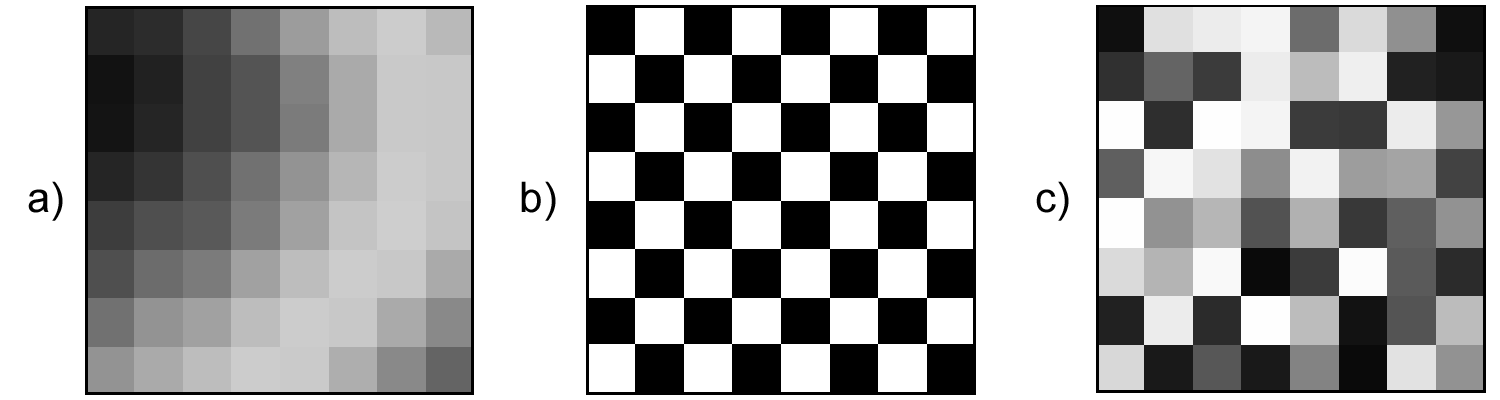
\includegraphics[width=\textwidth]{../es/Analisis/Autocorrelacion_espacial.png}
\caption{\small a) Autocorrelaci?n espacial positiva. b) Autocorrelaci?n espacial negativa. c) Ausencia de autocorrelaci?n espacial (independencia)}
\label{Fig:Autocorrelacion_espacial} 
\end{figure}

Las consecuencias de la existencia de autocorrelaci?n espacial son numerosas y de gran importancia.

Por una parte, muchos de los an?lisis estad?sticos suponen la \textbf{independencia de la variable}. Puesto que existe una dependencia de la componente espacial, ser? necesario para obtener resultados correctos introducir dicha componente espacial como una variable m?s. 

Algo similar sucede cuando los datos presentan alguna \textbf{tendencia espacial} (los valores de una variable est?n relacionados con sus propias coordenadas geogr?ficas), ya que esto tambien invalida el supuesto de la independencia de los datos.

Existiendo autocorrelaci?n espacial, y siendo esta positiva, la \textbf{inferencia estad?stica es menos eficaz} que si se cuenta con un n?mero igual de observaciones de una variable independiente. 

La autocorrelaci?n espacial no es, no obstante, un elemento que siempre tenga consecuencias negativas. Puesto que los puntos cercanos a uno dado guardan relaci?n con este, la autocorrelaci?n puede aprovecharse para \textbf{estimar valores} en un punto cualquiera si conocemos los valores en puntos cercanos. Este es el fundamento de los \textbf{m?todos de interpolaci?n}


\subsection{Existencia de estructura}

Tanto la disposici?n de los datos como las propiedades de la variable estudiada (por ejemplo, la propia autocorrelaci?n espacial como propiedad intr?nseca) exhiben una estructura determinada. Esta estructura puede condicionar los resultados del an?lisis y tener influencia sobre estos.

Los dos principales conceptos estad?sticos que definen la estructura espacial de los datos son la \textbf{estacionaridad} y la \textbf{isotrop?a}. La estacionaridad indica que el proceso es \textbf{invariante a la traslaci?n}. Es decir, que las propiedades son constantes en el espacio y no existe tendencia alguna. La isotrop?a indica que el proceso es \textbf{invariante a la rotaci?n} y tiene lugar del mismo modo en todas direcciones. 


\subsection{Efectos de borde}


Las zonas que estudiamos dentro de todo an?lisis espacial \textbf{tienen unos l?mites establecidos}. Estos l?mites vienen definidos de forma artificial ---el l?mite de la fotograf?a a?rea de la que disponemos, por ejemplo--- o bien de forma natural ---si estudiamos un bosque junto a un pantano, el bosque encuentra su l?mite al borde de este ?ltimo---. La presencia de estos bordes \textbf{distorsiona el resultado de los an?lisis}, en especial para aquellos par?metros no puntuales que requieren la definici?n de un area de estudio (densidades, etc., como ya vimos para el caso del PUAM)

En algunos casos, el efecto de borde no se manifiesta ?nicamente para puntos cercanos a dicho borde, sino para \textbf{todos aquellos relacionados o conectados} con ?l seg?n un determinado criterio, con independencia de su distancia a este.


\pagestyle{empty}